\documentclass[12pt,a4paper]{article}

% ─── Page Layout ───────────────────────────────────────────────────────────────
\usepackage[a4paper, margin=0.8in, headheight=14pt]{geometry}

% ─── Fonts (XeLaTeX) ───────────────────────────────────────────────────────────
\usepackage{fontspec}
\usepackage{unicode-math}
\setmainfont{TeX Gyre Pagella}
\setmonofont[Scale=0.88]{TeX Gyre Cursor}
\setmathfont{Latin Modern Math}

% ─── Packages ──────────────────────────────────────────────────────────────────
\usepackage{xcolor}
\usepackage{colortbl}
\usepackage{titlesec}
\usepackage{enumitem}
\usepackage{tabularx}
\usepackage{longtable}
\usepackage{booktabs}
\usepackage{array}
\usepackage{amsmath}
\usepackage{tikz}
\usetikzlibrary{shapes.geometric, arrows.meta, positioning, calc, fit, decorations.pathreplacing, patterns}
\usepackage{tcolorbox}
\tcbuselibrary{skins, breakable}
\usepackage{hyperref}
\usepackage{fancyhdr}
\usepackage{graphicx}
\usepackage{microtype}
\hyphenpenalty=10000
\exhyphenpenalty=10000
\sloppy
\usepackage{caption}
\usepackage{setspace}
\usepackage{multirow}
\usepackage{tocloft}

% ─── Q&A helper ────────────────────────────────────────────────────────────────
\newcommand{\Q}[1]{\textbf{#1}\par\noindent\ignorespaces}

% ─── Colour Palette ────────────────────────────────────────────────────────────
\definecolor{myred}{RGB}{196,30,58}
\definecolor{mydark}{RGB}{30,30,50}
\definecolor{mygreen}{RGB}{14,120,80}
\definecolor{myteal}{RGB}{0,130,140}
\definecolor{myamber}{RGB}{180,100,0}
\definecolor{mypurple}{RGB}{100,30,160}
\definecolor{mygray}{RGB}{246,247,249}
\definecolor{mgframe}{RGB}{180,185,200}
\definecolor{watermark}{RGB}{145,150,170}
\definecolor{hdrred}{RGB}{250,232,235}
\definecolor{hdrgreen}{RGB}{220,244,233}
\definecolor{hdrteal}{RGB}{220,242,244}
\definecolor{hdramber}{RGB}{253,242,215}
\definecolor{hdrpurple}{RGB}{238,228,255}
\definecolor{hdrgray}{RGB}{238,240,245}

% ─── Section Formatting ────────────────────────────────────────────────────────
\titleformat{\section}
  {\large\bfseries\color{myred}}{\thesection.}{0.5em}{}
  [\vspace{1pt}{\color{myred}\rule{\linewidth}{0.8pt}}]
\titleformat{\subsection}
  {\normalsize\bfseries\color{myteal}}{\thesubsection}{0.5em}{}
\titlespacing*{\section}{0pt}{18pt}{7pt}
\titlespacing*{\subsection}{0pt}{11pt}{4pt}

% ─── Paragraph ─────────────────────────────────────────────────────────────────
\setlength{\parindent}{0pt}
\setlength{\parskip}{4pt}

% ─── TOC Styling ───────────────────────────────────────────────────────────────
\renewcommand{\cfttoctitlefont}{\large\bfseries\color{myred}}
\renewcommand{\cftaftertoctitle}{\par\noindent{\color{myred}\rule{\linewidth}{0.8pt}}}
\setlength{\cftbeforetoctitleskip}{0pt}
\setlength{\cftaftertoctitleskip}{6pt}
\renewcommand{\cftsecfont}{\normalsize\bfseries\color{mydark}}
\renewcommand{\cftsecpagefont}{\normalsize\bfseries\color{mydark}}
\renewcommand{\cftsecleader}{\cftdotfill{\cftdotsep}}
\setlength{\cftbeforesecskip}{7pt}
\renewcommand{\cftsubsecfont}{\small\color{mydark}}
\renewcommand{\cftsubsecpagefont}{\small\color{mydark}}
\setlength{\cftbeforesubsecskip}{3pt}
\setlength{\cftsubsecindent}{1.4em}

% ─── Table helpers ─────────────────────────────────────────────────────────────
\renewcommand{\arraystretch}{1.45}
\setlength{\tabcolsep}{6pt}
\arrayrulecolor{mydark}
\newcolumntype{B}[1]{>{\small\bfseries\raggedright\arraybackslash}m{#1}}
\newcolumntype{Y}{>{\small\raggedright\arraybackslash}X}
\renewcommand{\tabularxcolumn}[1]{m{#1}}

% ─── Header / Footer ───────────────────────────────────────────────────────────
\pagestyle{fancy}
\fancyhf{}
\fancyhead[L]{\small\color{myred}\textbf{BS-B401}\;\color{mydark}--- Biology for Engineers}
\fancyhead[R]{\small\color{myteal}\textbf{Module 6 Notes}}
\fancyfoot[C]{\small\color{mydark}\thepage}
\fancyfoot[R]{\small\color{watermark}\textit{\copyright\ Biraj Sarkar (CGEC)}}
\renewcommand{\headrulewidth}{0.5pt}
\renewcommand{\footrulewidth}{0.3pt}

% ─── Hyperref ──────────────────────────────────────────────────────────────────
\hypersetup{
  colorlinks=true, linkcolor=myteal, urlcolor=myteal,
  pdfauthor={Biraj Sarkar (CGEC)},
  pdftitle={BS-B401 --- Module 6 Notes: Information Transfer}
}

% ─── tcolorbox styles ──────────────────────────────────────────────────────────
\tcbset{
  tikzbox/.style={
    colback=mygray, colframe=mgframe, boxrule=0.6pt, arc=4pt,
    left=8pt, right=8pt, top=6pt, bottom=6pt,
    colbacktitle=mgframe, coltitle=mydark, fonttitle=\small\bfseries
  },
  defbox/.style={
    colback=hdrgreen, colframe=mygreen, boxrule=0.8pt, arc=4pt,
    left=9pt, right=9pt, top=6pt, bottom=6pt,
    colbacktitle=mygreen, coltitle=white, fonttitle=\small\bfseries
  },
  formulabox/.style={
    colback=hdrteal, colframe=myteal, boxrule=0.8pt, arc=4pt,
    left=9pt, right=9pt, top=7pt, bottom=7pt,
    colbacktitle=myteal, coltitle=white, fonttitle=\small\bfseries
  },
  examplebox/.style={
    colback=hdramber, colframe=myamber, boxrule=0.8pt, arc=4pt,
    left=9pt, right=9pt, top=6pt, bottom=6pt,
    colbacktitle=myamber, coltitle=white, fonttitle=\small\bfseries
  },
  masonbox/.style={
    colback=hdrpurple, colframe=mypurple, boxrule=0.8pt, arc=4pt,
    left=9pt, right=9pt, top=6pt, bottom=6pt,
    colbacktitle=mypurple, coltitle=white, fonttitle=\small\bfseries
  },
  exambox/.style={
    colback=hdrpurple, colframe=mypurple, boxrule=1pt, arc=5pt,
    left=10pt, right=10pt, top=8pt, bottom=8pt,
    colbacktitle=mypurple, coltitle=white, fonttitle=\bfseries,
    breakable, title after break={\textbf{Frequently Asked / Viva Questions (contd.)}}
  }
}
\tcbset{breakable}
\tcbset{after={\par\color{black}}}

% ─── TikZ styles ───────────────────────────────────────────────────────────────
\tikzset{
  block/.style={rectangle, draw=myteal, fill=hdrteal,
    text width=2.4cm, align=center, minimum height=0.95cm,
    font=\small, rounded corners=3pt, line width=0.7pt},
  redblock/.style={rectangle, draw=myred, fill=hdrred,
    text width=2.4cm, align=center, minimum height=0.95cm,
    font=\small, rounded corners=3pt, line width=0.7pt},
  amberblock/.style={rectangle, draw=myamber, fill=hdramber,
    text width=2.4cm, align=center, minimum height=0.95cm,
    font=\small, rounded corners=3pt, line width=0.7pt},
  sumjunc/.style={circle, draw=myamber, fill=hdramber,
    minimum size=0.62cm, font=\small, line width=0.8pt},
  arrow/.style={-Stealth, thick, color=mydark},
  redarrow/.style={-Stealth, thick, color=myred},
  line/.style={thick, color=mydark}
}

\begin{document}

% ─── Title Page ───────────────────────────────────────────────────────────────
\begin{center}
  {\LARGE\bfseries\color{myred} BS-B401 --- Biology for Engineers}\\[5pt]
  {\normalsize\color{mydark} Semester IV \quad$\bullet$\quad 2L:1T:0P \quad$\bullet$\quad 3 Credits}\\[3pt]
  {\normalsize\color{myteal}\textbf{Module 6 Exam Notes: Information Transfer}}\\[3pt]
  {\small\color{mydark} CGEC \;$|$\; B.Tech ECE (2023--27) \;$|$\; \textit{Biraj Sarkar}}
\end{center}
\vspace{2pt}
\noindent{\color{myred}\rule{\linewidth}{1.5pt}}
\vspace{2pt}

\hypersetup{linkcolor=mydark}
\tableofcontents
\hypersetup{linkcolor=myteal}
\newpage

\section{Information Transfer}
\subsection{Evidence that DNA carries hereditary information}
\begin{tcolorbox}[defbox, title={Hereditary material}]
A hereditary molecule stores information, can be copied, can vary, and can be transmitted. DNA is the hereditary material of cellular organisms. Some viruses use RNA as their genome.
\end{tcolorbox}

\par\vspace{5pt}
\begingroup
\setlength{\extrarowheight}{1pt}
\noindent\begin{tabularx}{\linewidth}{|B{3.5cm}|Y|Y|}
\hline
\textbf{Study} & \textbf{Observation in outline} & \textbf{Interpretation} \\ \hline
Avery, MacLeod and McCarty & A DNA-containing fraction carried a heritable change. Degrading DNA removed that effect. & DNA could transmit a characteristic to descendant cells. \\ \hline
Hershey and Chase & The label associated with genetic material entering the host was chiefly linked to DNA rather than to the viral coat. & DNA carried the genetic instructions in the system studied. \\ \hline
\end{tabularx}\par
\endgroup
\subsection{DNA structure from strand to nucleosome}
\begin{enumerate}[leftmargin=*, itemsep=3pt, topsep=4pt]
  \item \textbf{One strand.} Deoxyribonucleotides are connected by $3'$--$5'$ phosphodiester bonds. The sugar-phosphate backbone is directional and the sequence of bases carries information.
  \item \textbf{Double helix.} Two complementary strands run antiparallel. A pairs with T and G with C through hydrogen bonding. Base stacking also stabilises the helix.
  \item \textbf{Nucleosome.} In eukaryotic chromatin, roughly 147 base pairs of DNA wrap around a histone octamer. Linker DNA lies between nucleosome core particles.
  \item \textbf{Chromatin.} Nucleosomes and associated proteins organise DNA further. Packaging influences accessibility for transcription and replication.
\end{enumerate}
\begin{tcolorbox}[tikzbox, title={Levels of eukaryotic DNA packaging}]
\centering
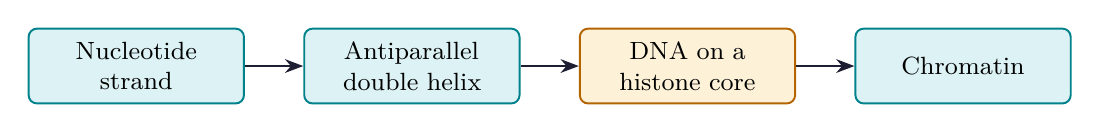
\begin{tikzpicture}[every node/.style={font=\small}]
\node[block,text width=2.5cm] (a) at (0,0) {Nucleotide\\strand};
\node[block,text width=2.5cm] (b) at (3.5,0) {Antiparallel\\double helix};
\node[amberblock,text width=2.5cm] (c) at (7,0) {DNA on a\\histone core};
\node[block,text width=2.5cm] (d) at (10.5,0) {Chromatin};
\draw[arrow] (a)--(b);
\draw[arrow] (b)--(c);
\draw[arrow] (c)--(d);
\end{tikzpicture}\par
\end{tcolorbox}

\section{Expression and the Genetic Code}
\subsection{Replication, transcription and translation}
\par\vspace{5pt}
\begingroup
\setlength{\extrarowheight}{1pt}
\noindent\begin{tabularx}{\linewidth}{|B{3.2cm}|Y|Y|}
\hline
\textbf{Process} & \textbf{Information direction} & \textbf{What to remember} \\ \hline
Replication & DNA to DNA. & Complementarity allows semiconservative copying. Each new duplex has one old strand and one new strand. \\ \hline
Transcription & DNA to RNA. & RNA polymerase reads a template strand and makes complementary RNA. The coding strand matches the transcript over the copied region apart from T versus U. \\ \hline
Translation & mRNA to polypeptide. & The ribosome reads codons. Transfer RNAs match the code and bring amino acids. \\ \hline
\end{tabularx}\par
\endgroup
\begin{tcolorbox}[masonbox, title={Follow direction carefully}]
RNA is synthesised $5'$ to $3'$. A template read in the opposite direction is complementary to the new RNA. Translation reads mRNA from $5'$ to $3'$ and extends a polypeptide from its N terminus to its C terminus.
\end{tcolorbox}

\subsection{What a codon specifies}
\begin{tcolorbox}[defbox, title={Genetic code}]
The genetic code maps each three-base mRNA codon to an amino acid or to a termination signal. A reading frame determines which groups of three are interpreted as codons.
\end{tcolorbox}

\begin{itemize}[leftmargin=*, itemsep=3pt, topsep=4pt]
  \item \textbf{Count.} Four possible RNA bases give $4^3=64$ codons. In the standard code, 61 specify amino acids and UAA, UAG and UGA signal termination.
  \item \textbf{Start.} AUG is the usual start signal in the correct initiation context. In an internal position it typically specifies methionine.
  \item \textbf{Degeneracy.} Several codons can specify the same amino acid. For example, GGU and GGC both specify glycine in the standard code.
  \item \textbf{Near universality.} The standard code is shared widely. Some mitochondria and organisms reassign particular codons, so the code is nearly universal.
  \item \textbf{Reading frame.} During ordinary translation, codons are read consecutively in the chosen frame. A one-base insertion or deletion can change downstream codons.
\end{itemize}
\begin{tcolorbox}[examplebox, title={Read a short illustrative message}]
For the classroom example $5'$--AUG GGU GAA UAA--$3'$, read AUG as the start and methionine, GGU as glycine and GAA as glutamate. UAA ends translation. The peptide is Met--Gly--Glu. The stop signal contributes no amino acid.
\end{tcolorbox}

\subsection{Gene as a functional and a recombination unit}
\begin{itemize}[leftmargin=*, itemsep=3pt, topsep=4pt]
  \item \textbf{Cistron.} In the classical functional definition, mutations that fail to complement in trans are usually assigned to the same functional unit. Mutations in different units may complement if each copy supplies the other's missing function.
  \item \textbf{Cis versus trans.} If two recessive mutations lie on one chromosome in cis, the opposite copy can carry both normal functions. In trans, the mutations lie on opposing copies. Restoration depends on whether functional copies of all required units are present.
  \item \textbf{Recon.} The classical recombination unit is the smallest genetic interval distinguishable by recombination in a given analysis. Recombination can separate sites inside one cistron, so a functional unit may contain many distinguishable sites.
  \item \textbf{Modern interpretation.} A gene is a DNA region contributing to a functional RNA or polypeptide. Regulatory and processing signals help specify when and how that product is made.
\end{itemize}

\subsection{Explain information flow in three stages}
\par\vspace{6pt}
\noindent\begin{tabularx}{\linewidth}{|B{3.1cm}|Y|Y|}
\hline
\textbf{Process} & \textbf{Start and extend} & \textbf{Finish or check} \\ \hline
Replication & Pair each parental strand with a new complementary strand. Both new strands extend in the same chemical direction, although the parental templates are antiparallel. & Each completed duplex retains one old strand. \\ \hline
Transcription & A promoter helps specify where transcription begins. RNA polymerase reads the selected DNA template and grows RNA in the $5'$ to $3'$ direction. & When transcription terminates, the RNA transcript is released. In eukaryotes a precursor transcript may be processed before use. \\ \hline
Translation & Initiation selects a start and fixes the reading frame. During elongation, transfer RNAs bring amino acids and the ribosome joins them. & A stop codon is read by a release factor in ordinary termination, releasing the polypeptide. \\ \hline
\end{tabularx}\par

\begin{tcolorbox}[examplebox, title={Use base pairing to check DNA composition}]
In an ordinary double-stranded DNA sample, suppose adenine makes up 28\% of the bases. Thymine also accounts for 28\%, leaving 44\% for guanine and cytosine together, or 22\% each. The calculation uses pairing across both strands. One individual strand need not have equal amounts of A and T.
\end{tcolorbox}

\subsection{Connect DNA packaging to gene accessibility}
\begin{itemize}[leftmargin=*, itemsep=2pt]
  \item \textbf{Core histones.} The nucleosome octamer contains two copies each of H2A, H2B, H3 and H4. DNA wraps around it, reducing the space needed to package a long molecule.
  \item \textbf{Linker DNA.} Short DNA segments connect successive core particles. Linker histone H1 can associate with this region and help organise chromatin.
  \item \textbf{Accessibility.} Packaging changes how readily proteins contact DNA. This can affect gene expression without changing the sequence of DNA bases.
\end{itemize}

\textbf{Structural reference.} \href{https://www.nature.com/articles/38444}{Luger et al., nucleosome core structure}.
\begin{tcolorbox}[masonbox, title={Keep the three meanings distinct}]
A codon is a triplet read during translation. A cistron is the classical functional unit inferred through complementation. A recon describes resolution in a recombination analysis. Several distinguishable recombination sites may lie within a single functional unit.
\end{tcolorbox}

\newpage
\begin{center}
  {\large\bfseries\color{myred} Quick Revision --- Module 6}\\[3pt]
  {\small\color{mydark} Information Transfer $|$ BS-B401}
\end{center}
\noindent{\color{myred}\rule{\linewidth}{1.2pt}}\par\vspace{4pt}

\begin{tcolorbox}[formulabox, title={Key Concepts at a Glance}]
\renewcommand{\arraystretch}{1.35}
\noindent\begin{tabularx}{\linewidth}{B{4.5cm}Y}
DNA pairing & A--T and G--C, with antiparallel backbones. \\[3pt]
Direction & DNA/RNA synthesis extends the $3'$ end. \\[3pt]
Code & 64 triplets, including three stop codons in the standard code. \\[3pt]
\end{tabularx}\par
\end{tcolorbox}

\begin{tcolorbox}[defbox, title={One-Line Definitions}]
\begin{itemize}[leftmargin=*, itemsep=3pt, topsep=4pt]
  \item \textbf{Codon.} Three-base mRNA unit interpreted during translation.
  \item \textbf{Nucleosome.} DNA wrapped around a histone core.
  \item \textbf{Cistron.} A classical functional unit defined by complementation.
\end{itemize}
\end{tcolorbox}

\begin{tcolorbox}[exambox, title={Frequently Asked / Viva Questions}]
\begin{enumerate}[topsep=0pt, label=\textbf{Q\arabic*.}, itemsep=5pt, leftmargin=*]
  \item \Q{What did the DNA-fraction study establish?}
    DNA could carry a heritable difference in the studied system.
  \item \Q{What does antiparallel mean?}
    The two strands have opposite backbone directions.
  \item \Q{How is DNA first compacted around histones?}
    It wraps around a histone octamer in the nucleosome core.
  \item \Q{Which process makes RNA from a DNA template?}
    Transcription.
  \item \Q{What does tRNA do?}
    It couples codon recognition to delivery of an amino acid.
  \item \Q{Which direction is mRNA read?}
    From $5'$ to $3'$.
  \item \Q{What does degeneracy mean?}
    More than one codon can specify the same amino acid.
  \item \Q{Is the code identical in every biological context?}
    Some organelles and organisms use codon reassignments.
  \item \Q{What is a frameshift?}
    A change in the grouping of downstream codons.
  \item \Q{Can a functional gene contain more than one recombination site?}
    Yes. Recombination can distinguish sites within a cistron.
\end{enumerate}
\end{tcolorbox}

\begin{tcolorbox}[tikzbox, title={Summary Comparison}]
\par\vspace{5pt}
\begingroup
\setlength{\extrarowheight}{1pt}
\noindent\begin{tabularx}{\linewidth}{|B{3.45cm}|Y|Y|}
\hline
\textbf{Process} & \textbf{Template or input} & \textbf{Main output} \\ \hline
Replication & DNA & DNA. \\ \hline
Transcription & DNA & RNA. \\ \hline
Translation & mRNA and amino acids & Polypeptide. \\ \hline
\end{tabularx}\par
\endgroup
\end{tcolorbox}

\end{document}
